\chapter{Grundlagen}\label{chap:fundamentals}

%\begin{itemize}
%%	\item evtl Section o.ä. zu Angriffen auf nicht DP-Federated Learning, bzw. warum braucht es DP auch im FL?
%	\item IDP-Teil nach Related Work?
%\end{itemize}

In diesem Kapitel gehe ich auf die Grundlagen ein, die für meine Arbeit wichtig sind. Zunächst gebe ich einen Überblick zu \textit{Differential Privacy}, beschreibe die fundamentale Idee, formalisiere sie und umreiße die wichtigsten Mechanismen, um sie anzuwenden. Danach führe ich Federated Learning ein, erwähne Probleme, die das Verfahren bei verzerrten Datenverteilungen hat und gehe auf mögliche Privatheitsmodelle im Federated Learning ein.

\section{Differential Privacy}

%\begin{itemize}
%%	\item Anwendung von DP in the wild (\cite{erlingsson:2014, tezapsidis:2017, apple:2017}) -> steht in introduction
%	\item Randomized Response als anschauliches Beispiel? (ähnlich wie bei \cite[p.1]{erlingsson:2014}) 
%\end{itemize}

\textit{Differential Privacy} ist ein Verfahren, das die Privatheit der Ergebnisse von interaktiven Anfragen auf Datenbanken schützt. Anders als bei nicht-interaktiven Privatheitsmaßen wie \textit{k-anonymity}, wird die Datenbank selbst dabei nicht verändert. Stattdessen werden Anfragen so abgewandelt, dass der Einfluss von individuellen Daten auf das Ergebnis klein wird, aber Trends in der gesamten Datenbank erkennbar bleiben.

Diese Idee wurde von \textcite{dwork:2006} formalisiert, nachdem sie zeigte, dass Anforderungen an Privatheit von \textcite{dalenius:1977} in der Praxis nicht umsetzbar sind. \citeauthor{dalenius:1977} war der Ansicht, dass ein Angreifer nichts über ein Individuum lernen soll, was er auch nicht auch ohne Zugriff auf die Datenbank hätte lernen können. \citeauthor{dwork:2006} zeigt, dass diese Vorgabe aufgrund von Hilfsinformationen, die der Angreifer besitzen kann, nicht umsetzbar ist. 

In einem Beispiel von \citeauthor{dwork:2006} gibt es eine Datenbank, aus der die durchschnittliche Größe von litauischen Frauen hervorgeht. Die Größe der Individuen wird als sensible Information betrachtet. Wenn der Angreifer die Hilfsinformation hat \glqq{}Person X ist zwei Zentimeter kleiner als der Durchschnitt litauischer Frauen\grqq{}, dann lernt er die genaue Größe von Person X, unabhängig davon, ob sie in der Datenbank ist oder nicht. 

Stattdessen verfolgt \citeauthor{dwork:2006} mit der \textit{Differential Privacy} einen Ansatz, bei dem nicht das Wissen des Angreifers einbezogen wird, sondern ob der Angreifer bei einer bestimmten Anfrage mehr über ein Individuum lernen kann, wenn es Bestandteil der zugrundeliegenden Datenbank ist.

Formal vergleicht \textit{Differential Privacy} die Wahrscheinlichkeit ein ähnliches Anfrageergebnis zu erhalten, wenn ein Individuum in einer Datenbank ist oder eben nicht. Je näher diese Wahrscheinlichkeiten beieinander liegen, desto weniger kann ein Angreifer durch die Präsenz des Individuums in der Datenbank lernen und desto höher ist die Privatheit. Die Definition aus \cite{dwork:2006} ist folgende:

\begin{definition}\label{def:eps-differential-privacy}
	\emph{\textbf{$\epsilon$-Differential Privacy}} Ein \textit{Zufallsmechanismus} $\mathcal{M}: \mathcal{D} \rightarrow \mathcal{R}$ mit der Domäne $\mathcal{D}$ und dem Wertebereich $\mathcal{R}$ erfüllt $\epsilon$-Differential Privacy wenn für zwei beliebige benachbarte Eingaben $d$, $d' \in \mathcal{D}$ jede Teilmenge von Ausgaben $S \subseteq \mathcal{R}$ gilt, dass $$\Pr[\mathcal{M}(d) \in S] \leq e^{\epsilon} \Pr[\mathcal{M}(d') \in S]$$
\end{definition}

Hervorzuheben ist hierbei, dass die Definition fast keine Anforderungen an die Datenbanken $d$ und $d'$ stellt, außer, dass sie benachbart sind. Typischerweise gilt dafür die folgende Definition:
% Quelle hinzufügen? Bzw. klar machen warum ich sie hier explizit aufschreibe, nämlich in abgrenzung zu den User-adjacent datasets\cite{mcmahan:2018}
\begin{definition}\label{def:example-adjacency}
	\emph{\textbf{Example-adjacent datasets}} Zwei Datensätze $d$ und $d'$ sind als example-adjacent definiert, wenn $d'$ erzeugt werden kann, indem ein einzelnes Beispiel aus $d$ gelöscht oder $d$ hinzugefügt wird.
\end{definition}

Wenn in dieser Arbeit von benachbarten Datensätzen die Rede ist, gilt i.A. diese Definition, wenn nicht explizit anders beschrieben.

Eine leicht abgeschwächte Version der Definition fügt einen Parameter $\delta$ hinzu, der die Wahrscheinlichkeit repräsentiert, dass die Privatheitsgarantien nicht eingehalten werden. Er sollte dementsprechend sehr klein gewählt werden \cite{dwork:2014}. Diese Definition ist relevant, da der häufig verwendete \textit{Gaussian Mechanism} die strengere $\epsilon$-\textit{Differential Privacy} Definition nicht erfüllt, man aber trotzdem mit ihm arbeiten will. Außerdem ist er für das \textit{Advanced Composition Theorem} notwendig.

\begin{definition}\label{def:eps-delta-differential-privacy}
	\emph{\textbf{$(\epsilon, \delta)$-Differential Privacy}} Ein \textit{Zufallsmechanismus} $\mathcal{M}: \mathcal{D} \rightarrow \mathcal{R}$ mit Domäne $\mathcal{D}$ Wertebereich $\mathcal{R}$ erfüllt $(\epsilon, \delta)$-Differential Privacy wenn für zwei beliebige benachbarte Eingaben $d$, $d' \in \mathcal{D}$ und für jede Teilmenge der Ausgaben $S \subseteq \mathcal{R}$ erfüllt ist, dass $$\Pr[\mathcal{M}(d) \in S] \leq e^{\epsilon} \Pr[\mathcal{M}(d') \in S] + \delta$$
\end{definition}

Darüber hinaus gibt es noch die Rényi-\textit{Differential Privacy}, die neben dem $\epsilon$ noch einen Parameter $\alpha$ hat. Sie ist für viele Theoreme wichtig, ist aber weniger anschaulich und kann immer in $(\epsilon, \delta)$-Differential Privacy überführt werden, weshalb ich hier nicht weiter auf diese Definition eingehen werde. Es gilt, dass ein Mechanismus, der $(\alpha, \epsilon)$-DP erfüllt auch immer $(\epsilon', \delta')$-DP erfüllt für $0 < \delta' < 1$ und $\epsilon' = \epsilon + \frac{\log 1 / \delta'}{\alpha - 1}$ \cite{mironov:2017}.

Um eine Anfrage nach der Definition von \textit{Differential Privacy} privat zu machen, wird auf ein Anfrageergebnis von $\mathcal{M}$ Rauschen hinzugefügt. Das Rauschen kann beispielsweise aus der Laplace- oder der Normalverteilung gezogen werden. Die Varianz der Verteilung, aus der das Rauschen gezogen wird hängt von der Sensitivität einer Anfrage ab. Sie beschreibt die größtmögliche Veränderung des Anfrageergebnisses, die durch das Hinzufügen oder das Löschen eines Eintrags auftreten kann \cite{dwork:2006}.

\begin{definition}\label{def:l1-sensitivity}
	\emph{\textbf{L1-Sensitivity}} Für $\mathcal{M}: \mathcal{D} \rightarrow \mathcal{R}^{d}$, ist die L1-Sensitivität von $\mathcal{M}$
	$$
	\Delta \mathcal{M} = \max_{d_1, d_2}{||\mathcal{M}(d_1) - \mathcal{M}(d_2)||}_1
	$$
	für alle benachbarten Datensätze $d_1$, $d_2$
\end{definition}

Die Verteilungen werden je nach Anwendungsfall gewählt. Beispielsweise gibt es den Laplace- oder den Gauss'schen Mechanismus, um numerische Anfragen, beispielsweise Durchschnitt einer Datenbank, privat zu machen. Für Anfragen, die ein Ergebnis aus einer festgelegten Menge liefern sollen, gibt es den Exponentiellen Mechanismus. Dieser bewertet die potenziellen Ergebnisse anhand einer Bewertungsfunktion.\cite{mcsherry:2007}

Bei den Mechanismen variiert die Definition der Sensitivität leicht. Beispielsweise nutzt der Gauss'sche Mechanismus die $\ell_2$-Norm anstatt der $\ell_1$-Norm, die Intuition, dass es um die maximale Abweichung im Anfrageergebnis durch ein Individuum geht, bleibt jedoch immer erhalten. Darüber hinaus erfüllt der Laplace Mechanismus $\epsilon$-Differential Privacy, der Gauss'sche Mechanismus jedoch nur $(\epsilon, \delta)$-Differential Privacy.\cite[p.261ff]{dwork:2014}

Mit den bisher erwähnten Methoden kann die Privatheit einzelner Anfragen gewährleistet werden. Wenn aber mehrfach Anfragen gestellt werden, muss auch das Niveau der Privatheit abnehmen, da der Durchschnitt der einzelnen Anfragen irgendwann gegen den echten Wert konvergiert \cite[p.42]{dwork:2014}. Ein großer Vorteil von Differential Privacy ist, dass sich diese Verringerung der Privatheit abschätzen lässt. Dafür gibt es einige Kompositionstheoreme:

Das \textit{Basic Composition Theorem} sagt, dass die $k$-fache Anwendung von jeweils $\epsilon_i$-DP Mechanismen ein Privacy-Budget von $\epsilon = \sum_{i=1}^{k} \epsilon_i$ benötigt. Für die strenge $\epsilon$-DP Defintion ist das die optimale Abschätzung \cite{steinke:2022}. Allerdings wächst damit das Privacy Budget linear mit der Anzahl der Anfragen. 

Das Theorem lässt sich auch auf $(\epsilon, \delta)$-DP übertragen, allerdings gibt es dafür mit dem \textit{Advanced Composition Theorem} auch eine asymptotisch bessere Abschätzung. Details dazu sind in \textcite{dwork:2010, steinke:2022} zu finden.

Mechanismen, bei denen ein \textit{Subsampling} durchgeführt wird, also bei denen nur eine zufällige Teilmenge der Datenbank ausgewertet wird, können weitere Privacy Vorteile mit sich bringen \cite{mironov:2019, steinke:2022}.

Darüber hinaus können Ergebnisse, die durch einen Mechanismus erhalten wurden der Differential Privacy erfüllt, weiterverarbeitet werden, ohne dass die Privatheit weiter kompromittiert wird (\textit{post-processing}) \cite{dwork:2014}.

\subsection{Differential Privacy im Machine Learning}\label{sec:fund-dp-in-ml}

%\begin{itemize}
%%	\item Attacken auf Privatheit beschreiben, gegen die DP hilft? (wie in der Introduction von \cite{abadi:2016})
%%	\item Warum nutzt man DP, was ist die Motivation -> Verteidigung gegen Model Inversion Attacks(?), ...
%	\item was sind Variablen beim Training, die einen Einfluss auf das benötigte Privacy Budget haben? (Da kann dann eine Brücke zum FL geschlagen werden)
%\end{itemize}

Das Ziel von \textit{Differential Privacy} im \textit{Machine Learning} ist, die Privatheit der einzelnen Datenpunkte in den Trainingsdaten zu schützen. Es handelt sich in diesem Fall nicht um den Schutz der Datenbank, sondern es soll verhindert werden, dass sensible Informationen aus den Trainingsdaten bei der Nutzung des trainierten Modells durch Dritte gefunden werden können. 

% etwas zu reconstruction attacks
Angriffe auf Machine Learning Modelle sind beispielsweise \textit{Reconstruction Attacks}, \textit{Model Inversion Attacks} oder \textit{Membership Inference Attacks}. Bei \textit{Reconstruction Attacks} wird versucht anhand von Features Originaldaten wiederherzustellen. Auch wenn die meisten Machine Learning Algorithmen Features von Trainingsdaten nicht direkt speichern, gibt es einzelne Algorithmen wie Support Vector Machines die es doch tun und damit diesen Attacken ausgesetzt sein können \cite[p.9ff]{chang:2023}.

Bei \textit{Model Inversion Attacks} wird versucht, die Eingabe in ein Modell anhand der Ausgabe vorherzusagen. \textcite{fredrikson:2015} haben APIs von \textit{Machine Learning as a Service}-Anbietern analysiert und eine solche Attacke basierend auf den Antworten ihrer Modelle durchgeführt. Dazu haben sie KI-Modelle trainiert, die sensible Attribute aus Umfragen, aber auch Eingabebilder für eine Gesichtserkennung wiederherstellen konnten. Das hat insbesondere mit den Beispielen gut funktioniert, mit denen die Modelle der Anbieter trainiert wurden und stellt daher ein großes Risiko für Leute dar, die Trainingsdaten zu solchen Modellen beisteuern. Um die Effektivität der Attacke zu minimieren schlagen \citeauthor{fredrikson:2015} vor, den Detailgrad der Ausgabe zu verringern. Sie zeigen, dass das rekonstruierte Bild bei einer Gesichtserkennung deutlich schlechter wird, wenn die Wahrscheinlichkeiten, dass das Bild eine bestimmte Person darstellt, ausreichend gerundet wird. Alternativ kann auf die Ausgabe der Wahrscheinlichkeiten verzichtet werden und nur die wahrscheinlichste Klasse ausgegeben werden.

Insbesondere kann Differential Privacy die Effektivität von \textit{Membership Inference Attacks} \cite{shokri:2017} deutlich verringern \cite[p.14f]{chang:2023}. Das Ziel dieser Attacken ist nicht die Rekonstruktion von Eingabedaten, sondern aufgrund von Ausgaben eines trainierten Modells herauszufinden, ob ein Datenpunkt Teil der Trainingsdaten war.

Im Allgemeinen entsteht durch die Anwendung von Differential Privacy im Machine Learning ein Trade-Off zwischen der Nützlichkeit und der Privatheit des Modells (\textit{Privacy-Utility Trade-off}). Daher wird auf verschiedene Arten versucht dabei eine möglichst gute Nützlichkeit des Modells beizubehalten. Zum einen wird an besseren Abschätzungen der Privacy-Kosten geforscht \cite{dwork:2010, abadi:2016, mironov:2019}. Darüber hinaus werden Algorithmen entwickelt, die bessere Ergebnisse erzielen können als andere \cite{papernot:2017}. Es gibt auch Arbeiten, die sich mit der Modellarchitektur selbst beschäftigen. Beispielsweise haben \textcite{papernot:2021} den Effekt von Aktivierungsfunktionen auf Privacy Parameter erforscht und konnten mit beschränken Aktivierungsfunktionen neue \textit{State-of-the-art}-Genauigkeiten auf MNIST, FashionMNIST und CIFAR10 erzielen.

Eine weitere Forschungsrichtung ist die Anwendung von individuellen Privacy Budgets für einzelne Nutzer oder Datenpunkte. Sie kann sich auf empirische Studien stützen, die nahelegen, dass verschiedene Personen unterschiedliche Anforderungen an die Privatheit ihrer Daten haben \cite{jensen:2005, acquisti:2005}. In \autoref{fund-idp} und den weiteren Kapiteln werde ich diese Forschungsrichtung weiter beleuchten.

Im Training selbst gibt es verschiedene Punkte, an denen \textit{Differential Privacy} ansetzen kann, um die Privatheit zu gewährleisten. Jeder Punkt hat verschiedene Vor- und Nachteile, die ich im Folgenden umreiße. Eine Übersicht dazu ist in \autoref{fig:design_principles_dpml} zu sehen.

\begin{figure}[tb]
	\centering
	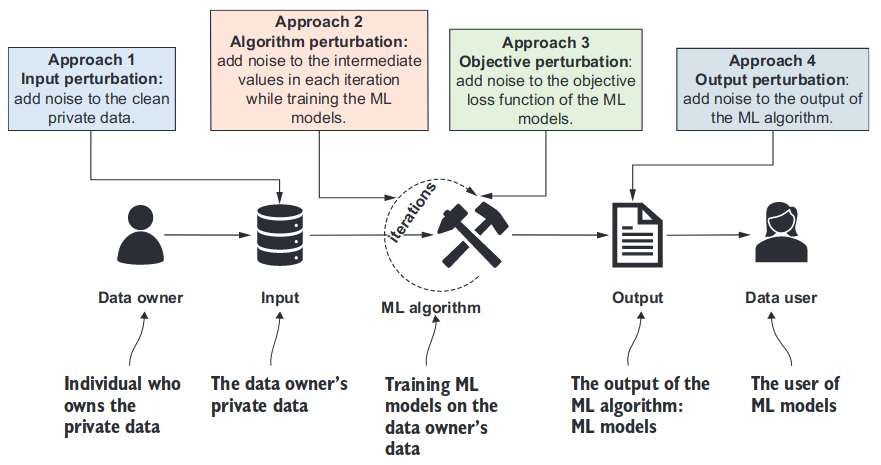
\includegraphics[width=0.9\textwidth]{Bilder/design_principles_dpml.png}
	\caption{Design Prinzipen im Machine Learning mit Differential Privacy aus \textcite{chang:2023}}
	\label{fig:design_principles_dpml}
\end{figure}

Bei der \textit{Input Pertubation} wird den Trainingsdaten Rauschen hinzugefügt, bevor das Modell mit ihnen trainiert wird. Dieser Ansatz ist ohne weitere Änderungen am Trainingsalgorithmus oder am Modell anwendbar, da der Trainingsalgorithmus dann Daten verarbeitet, die bereits differential private sind und es damit einem \textit{post-processing} entspricht. Das Modell kann danach also problemlos weiterverwendet werden. Ein großer Nachteil ist aber, dass die Anfragen auf den Trainingsdaten im Allgemeinen eine hohe Sensitivität haben und daher viel Rauschen hinzugefügt werden muss.

Die \textit{Algorithm Pertubation} ist das am weitesten verbreitete Verfahren und liegt großen Bibliotheken wie Opacus \cite{yousefpour:2021} und TensorFlow Privacy \cite{tfprivacy} zugrunde. Es kann für iterative Optimierungsverfahren wie Gradient Descent oder die Power Iteration Methode bei einer Principal Component Analysis (PCA) genutzt werden.

Bei der Anwendung dieses Verfahrens im \textit{Gradient Descent} wird \textit{Differential Privacy} auf die Gradienten angewendet, das heißt, diese werden für gewöhnlich auf eine bestimmte Vektornorm gestutzt und dann wird basierend darauf Rauschen addiert. In der Regel muss hierbei deutlich weniger Rauschen hinzugefügt werden als bei der \textit{Input Pertubation}.\cite{chang:2023} Der \textit{Privacy Loss}, der durch einen Trainingsdurchlauf anfällt, kann mithilfe von Kompositionstheoremen bestimmt werden. Für die Abschätzung wurde das \textit{Strong Composition Theorem}\cite{dwork:2010} genutzt, allerdings konnten \textcite{abadi:2016} mit dem \textit{Moments Accountant} eine deutlich genauere Abschätzung für das Training von Neuronalen Netzen liefern. So können Neuronale Netze mit dem Verfahren bereits mit kleinen Privacy Budgets trainiert werden. Das trainierte Modell kann ebenfalls veröffentlicht werden, da dessen Gewichte die Anforderungen der Differential Privacy erfüllen. Es schützt also insbesondere nicht nur davor, dass Anfragen an das Modell einem Angreifer Informationen geben können, sondern auch davor dass der Angreifer das Modell herunterlädt und beispielsweise die Modellparameter analysiert.

\textcite{shokri:2015} entwickelten bereits vor \textcite{abadi:2016} ein dezentrales Trainingsverfahren für Neuronale Netze unter Einhaltung von Differential Privacy. Ähnlich wie im Federated Learning (siehe \autoref{fund-fl}) schlagen sie ein verteiltes Training vor. In ihrem Protokoll werden von jedem Teilnehmer nur eine Teilmenge seiner Parameter geteilt, weshalb die Privacy-Budgets pro Modellparameter spezifiziert werden. Parameter, die einen größeren Gradienten als einen vorher spezifizierten Schwellwert haben, werden mit dem Laplace-Mechanismus verrauscht und dann an den Modell-Server geschickt. Die Summe der Privacy-Budgets für ein ganzes Modell kann allerdings sehr groß werden\cite[p.10]{abadi:2016}.

\textit{Objective Pertubation} verändert die Zielfunktion des Trainings. Statt auf die Daten wird während des Trainings Rauschen auf diese Funktion gelegt.

Bei der \textit{Output Pertubation} wird ein nicht-privates Modell trainiert und nur die Ausgabe des Modells verrauscht. Dieses Verfahren hat den großen Nachteil, dass es nicht anwendbar ist, wenn das Modell veröffentlicht werden soll.

Ein Vertreter dieses Ansatzes ist \textit{PATE}\cite{papernot:2017}. Hierbei werden \textit{Teacher Models} auf disjunkten Teilmengen der sensitiven Trainingsdaten trainiert. Das Ensemble dieser \textit{Teacher Models} trainiert danach ein \textit{Student Model} auf einem nicht-sensitiven oder öffentlichen Datensatz. Diese Daten müssen nicht gelabelt sein, da die trainierten \textit{Teacher Modelle} die Labels generieren. Vorteil dieses Verfahrens ist, dass es keine Anforderungen an die Modelle oder den Trainingsprozess stellt. Auch die \textit{Teacher Models} müssen nicht privat trainiert werden, denn die Privatheit entsteht dadurch, dass auf die Ausgabe des Ensembles mit dem \textit{Laplace Mechanismus} Rauschen hinzugefügt wird. Das entspricht der \textit{Output Pertubation}. Da die wiederholte Anfrage der \textit{Teacher Modelle} den Verlust an Privacy erhöht, wird nur eine vorher festgelegte Anzahl an ungelabelten Daten für das \textit{Student Model} mit Labels versehen. Dabei wird nur das mit der größten Konfidenz vorhergesagte Label genutzt. So lässt sich der \textit{Privacy Loss} mithilfe von Kompositionstheoremen abschätzen. Durch die verrauschten Vorhersagen der \textit{Teacher Modelle} wird das \textit{Student Model} privat trainiert und kann ohne Einschränkungen veröffentlicht werden.

Abgesehen von der Varianz des Laplaceschen Rauschens ist die Anzahl der \textit{Teacher Models} wichtig für den Trade-Off zwischen Privacy und Genauigkeit. Eine größere Anzahl an \textit{Teacher Models} verringert den Verlust an Privacy, allerdings wird auch deren Genauigkeit verringert, da die Menge der Trainingsdaten pro \textit{Teacher Model} abnimmt.

\textcite{papernot:2017} evaluieren \textit{PATE} auf MNIST und SVHN. Im Fall von SVHN nutzen sie die \textit{Extended Version} des Datensatzes und betonen, dass die größere verfügbare Menge an Trainingsdaten die zusätzliche Komplexität des Datensatzes kompensiert. Mit 250 \textit{Teacher Models} können sie Genauigkeiten von $98\%$ (MNIST) und $90.66\%$ (SVHN) erzielen. Das Ergebnis auf MNIST kann damit \textcite{abadi:2016} schlagen.

Der größte Nachteil an PATE ist, dass der Algorithmus nicht-private (potenziell ungelabelte) Daten benötigt, da das \textit{Student Model} nicht-privat trainiert wird. Diese Voraussetzung braucht der Algorithmus von \textcite{abadi:2016} nicht.

\subsection{Individualisierte Differential Privacy}\label{fund-idp}

Motiviert von den verschiedenen Anforderungen und Präferenzen unterschiedlicher Personen an die Privatheit ihrer Daten haben \textcite{alaggan:2016} und wenig später unabhängig \textcite{jorgensen:2015} Arbeiten zu \textit{Differential Privacy} mit individuellen \textit{Privacy Budgets} veröffentlicht.

\textcite{alaggan:2016} definieren heterogene Differential Privacy im Kontext von Nutzerprofilen. In ihrer Arbeit individualisieren sie die Privacy durch das Anpassen der Sensitivität der Komponenten mit unterschiedlichen Budgets. Dazu erstellen sie eine \textit{Shrinkage Matrix}, mit der die Datenpunkte multipliziert werden. Die Matrix ist eine Diagonalmatrix, bei der die Diagonalelemente in $[0;1]$ liegen und abhängig von dem jeweiligen Privacy Budget sind.

Ihr Ansatz ist jedoch für einige Funktionen nicht anwendbar, beispielsweise können das Minimum und die $\ell_0$-Norm nicht berechnet werden.

\textcite{jorgensen:2015} stellen einen Sampling Ansatz vor, mit dem beliebige DP-Algorithmen in einen Algorithmus mit individualisierter DP überführt werden können. Dabei wird der zugrundeliegende DP-Algorithmus als Black Box betrachtet und die Wahrscheinlichkeit, dass ein Tupel für den Algorithmus gezogen wird, davon abhängig gemacht, was der Nutzer als Privacy Budget gewählt hat.

In ihren Experimenten betrachten sie das gewählte Privacy Budget eines Nutzers als öffentliche Information. Dies kann als problematisch gewertet werden, da es theoretisch etwas über die Wichtigkeit einer Information aussagen kann. Sie rechtfertigen diesen Umstand damit, dass die Budgets nicht für ein Attribut gewählt werden, sondern für ein Individuum mit potenziell vielen Attributen. Diese Information sagt daher nur etwas über die Person aus. Sie plädieren außerdem dafür, einen Nutzer anstatt eines genauen Budgets eine bestimmte Privatheitsstufe mit angemessener Beschreibung (niedrig, mittel und hoch) angeben zu lassen, damit die Semantik der Budgets für Endnutzer verständlich bleibt.

Darüber hinaus zeigen sie ein weiteres Verfahren, das auf dem \textit{Exponential Mechanism} basiert. Diesen verändern sie so, dass die Score-Funktion die individuellen Privacy Budgets mitbetrachtet. Sie wenden diesen Mechanismus auf \textit{Count}, \textit{Median} und \textit{Min} an, merken aber an, dass das Finden eines Algorithmus, der die angepasste Score-Funktion für beliebige Funktionen effizient berechnet, nicht trivial ist.

Sie weisen die Effektivität ihrer Verfahren in Experimenten nach, in denen sie beide Verfahren für \textit{Count} und \textit{Median} und eine \textit{Multiple Linear Regression} nur mit dem Sampling-Verfahren durchführen. Ihr Vorgehen vergleichen sie mit Standard-DP-Verfahren und bei \textit{Count} zusätzlich mit den Stretching-Verfahren von \textcite{alaggan:2016}. Die Privacy Budgets teilen sie in drei Gruppen mit aufsteigenden Privacy-Budgets auf (\textit{conservative}, \textit{moderate} und \textit{liberal}). Bei \textit{Count} leidet das Sampling-Verfahren dadurch, dass Elemente augeschlossen werden. Allerdings kann der angepasste \textit{Exponential Mechanism} gute Ergebnisse liefern und das Stretching-Verfahren schlagen. \textit{Median} verhält sich gegenüber dem Sampling deutlich resistenter, weshalb der Ansatz hier auch gute Ergebnisse erzielen kann und auch besser abschneidet als der modifizierte \textit{Exponential Mechanism}. 

Auch bei der linearen Regression kann der Sampling Ansatz das Verfahren von \cite{alaggan:2016} schlagen. Der modifizierte \textit{Exponential Mechanism} ist hier nicht anwendbar.

\section{Federated Learning}\label{fund-fl}

Federated Learning (FL) ist ein Optimierungsverfahren, bei dem einzelne Clients gemeinsam über mehrere Runden ein Modell trainieren, ohne dabei ihre eigenen Trainingsdaten mit anderen zu teilen. Auch wenn noch viele Fragen im Federated Learning offen sind und erforscht werden, wird es erfolgreich in Produktivumgebungen eingesetzt und stellt im Training mit besonders sensiblen Daten eine gute Alternative gegenüber dem klassischen zentralisierten Training dar \cite{hard:2018, ramaswamy:2020}.

Im Federated Learning gibt es einen Server, der den Ablauf des Trainings steuert. Außerdem gibt es eine beliebige Anzahl von Clients, die das lokale Training auf ihren eigenen Daten durchführen. Der generelle Ablauf einer Trainingsrunde sieht wie folgt aus: 

\begin{enumerate}
	\item Der Server initialisiert ein Modell und dessen Parameter (nur erste Runde). 
	\item \label{round-start} Er wählt eine Menge von Clients aus, mit denen in dieser Runde das Modell trainiert werden soll.
	\item Das Modell wird an die ausgewählten Clients geschickt.
	\item Die Clients optimieren das Modell auf ihren eigenen Daten und schicken die aktualisierten Parameter zurück an den Server.
	\item Der Server aggregiert die Parameter der Clients und konstruiert daraus neue Modellparameter.
	\item Die nächste Runde beginnt mit \autoref{round-start}. Das Training endet, wenn das Modell konvergiert oder die festgelegte Rundenzahl erreicht ist.
\end{enumerate}

Die lokale Optimierung und die Aggregation der Updates variiert je nach Algorithmus. Die beiden Standardalgorithmen sind \texttt{FedAvg} und \texttt{FedSGD}\cite{mcmahan:2016}. Der wichtigste Unterschied zwischen ihnen ist, dass \texttt{FedAvg} die Clients mehrere Epochen auf ihren eigenen Daten trainieren lässt, während die Clients im \texttt{FedSGD} nur einen Schritt machen, bevor sie die aktualisierten Parameter wieder an den Server schicken. In beiden Algorithmen werden die Updates bei der Aggregation nach der Menge an Datenpunkten beim jeweiligen Client gewichtet.

Das verteilte Training kann vor allem zwei Probleme mit sich bringen: zunächst kann der Zusatzaufwand für die Kommunikation sehr groß werden, gerade wenn über viele Runden hinweg trainiert wird. Zum anderen kann nicht angenommen werden, dass die Daten über die Clients hinweg unabhängig und gleichverteilt (i.i.d.) sind, was die Konvergenz der Algorithmen beeinträchtigen kann. \textcite{karimireddy:2020} versuchen diesem Problem zu begegnen, indem sie in ihrem Algorithmus die generelle Richtung, in die die Clients optimieren, an die Clients schicken und diese sie in ihre Updates einfließen lassen.

Die Anwendungsfälle von Federated Learning können variieren: Zum einen gibt es das \textit{Cross-device Federated Learning} und zum anderen das \textit{Cross-silo Federated Learning}\cite{kairouz:2021}. 

Ersteres entspricht dem Fall, dass die Clients eine Vielzahl von mobilen Geräten oder IoT-Geräten sind. Hierbei sind die Clients sehr unzuverlässig, zum Beispiel kann sich der Empfang verschlechtern, ein Gerät ausgeschaltet werden oder das Gerät wegen einem zu niedrigen Akkustand ungeeignet für die Teilnahme am Training sein. All dies kann von dem Server nicht beeinflusst werden, also muss das Trainingsverfahren mit solchen Ausfällen zurecht kommen. Darüber hinaus kann die Menge der Clients von dem Server nicht verlässlich indiziert werden, da Geräte auch dauerhaft ausfallen können, zum Beispiel wenn ein Mobiltelefon kaputt geht oder ein neues gekauft wird und deshalb laufend neue Geräte hinzukommen können.

Bei dem \textit{Cross-silo Federated Learning} geht es vor allem um das Trainieren von Modellen zwischen unterschiedlichen Datencentern oder Organisationen. Die Motivation hierbei ist vor allem, dass es ein gemeinsames Interesse mehrerer Parteien an aussagekräftigen Modellen gibt, aber die zugrundeliegenden Trainingsdaten nicht den anderen Organisationen bereitgestellt werden sollen. Hierbei ist die Ausfallsicherheit der Clients deutlich höher als beim \textit{Cross-device Federated Learning} und die Menge der Clients ist in der Regel bekannt.

Auch der Server selbst kann bei einer sehr großen Zahl von Clients zu einem Engpass werden \cite[p.11]{kairouz:2021}. Daher wird ebenfalls an vollständig verteilten Trainingsverfahren geforscht, bei denen kein zentraler Server nötig ist (\textit{Fully-decentralized learning}).

\subsection{Datenheterogenität}\label{fund-fl-data-heterogenity}

Ein häufig beschriebenes Problem des Federated Learnings ist die Heterogenität der Trainingsdaten. Da die Daten von unterschiedlichen Parteien generiert werden, ist eine zufällige Verteilung der abhängigen und unabhängigen Variablen in der Regel nicht gegeben. Diese Heterogenität kann sich auf verschiedene Arten ausdrücken, wie im folgenden beschrieben.

Die Daten auf den einzelnen Clients können Abhängigkeiten aufweisen, beispielsweise wenn sie in einer zeitlichen Abfolge sortiert vorliegen. Derartige Abhängigkeiten können aber durch das Durchmischen der einzelnen Datenpunkte gelöst werden. Eine solche Verzerrung wird \textit{Intra-Client Distribution Skew} genannt.

Die Verteilung der \textit{Features} kann sich zwischen den Clients unterscheiden, auch wenn die Wahrscheinlichkeit der Labels gegeben der Features, $P(y|x)$, die gleiche ist. Beispielsweise könnte es sein, dass eine Person sehr viele Hundebilder auf ihrem Handy hat, weil sie einen Hund als Haustier hat. Eine andere Person hat sehr viele Katzenbilder auf ihrem Handy, weil sie mit einer Katze wohnt. Trotzdem wäre die Wahrscheinlichkeit, dass das Label bei einem Katzenbild auch Katze ist, die gleiche. Diese Art von Verzerrung heißt \textit{Feature Distribution Skew}.

Umgekehrt kann sich auch die Verteilung der Labels auf den Clients unterscheiden, zum Beispiel aufgrund von regionalen Unterschieden. Beispielsweise können Kängurus fast nur in Australien beobachtet werden. So ein Fall wird als \textit{Label Distribution Skew} bezeichnet.

Darüber hinaus werden von \textcite{kairouz:2021} weitere Verzerrungen erwähnt. So kann es sein, dass sich die bedingten Wahrscheinlichkeiten von Features und Labels unterscheiden, beispielsweise sieht ein Haus in den USA anders aus als ein Haus in Europa, in beiden Fällen ist es aber ein Haus (\textit{concept drift}). Andersherum kann es auch sein, dass die gleichen Features anders gelabelt sind, beispielsweise weil manche Daten auch für Menschen ununterscheidbar sind. Außerdem kann die Anzahl der Trainingsbeispiele von Client zu Client sehr stark variieren. 

\subsection{Privacy Model im Federated Learning}\label{sec:pm-in-fl}
Auch wenn das Training von Modellen im Federated Learning verhindert, dass Trainingsdaten das eigene Gerät verlassen, sind Angriffe auf die trainierten Modelle weiterhin möglich. Das schließt die in \autoref{sec:fund-dp-in-ml} beschriebenen Attacken ein. Es gibt auch weitere Arbeiten, die sich speziell mit Federated Learning befassen \cite{geiping:2020, wang:2019}. Die Anwendung von Differential Privacy im Federated Learning hat das Potenzial, die mit den Attacken verbundenen Risiken zu mindern. Es gibt unterschiedliche Herangehensweisen, um Differential Privacy im Federated Learning umzusetzen.

% local vs global (trusted server), record vs user level
Die bisherige Definition von Differential Privacy geht davon aus, dass die Privatheit einzelner Datenpunkte in einer Datenbank geschützt wird. Im Federated Learning ist die Struktur der Daten eine andere: Es gibt viele Clients und es ist wichtig die Privatheit des ganzen Datensatzes eines Clients zu schützen. Es reicht nicht aus einzelne Zeilen seiner Daten zu schützen. Wenn die Menge der Daten aller Clients als Datenbank angesehen wird, kann die Definition der benachbarten Datensätze aus  Defintion \autoref{def:example-adjacency} dementsprechend angepasst werden:

\begin{definition}\label{def:user-adjacency}
	\emph{\textbf{User-adjacent datasets} \cite{mcmahan:2018}} Seien $d$ und $d'$ zwei Datensätze mit Trainingsdaten, die jeweils mit einem Nutzer assoziiert sind. Dann sind $d$ und $d'$ benachbart (\textbf{user-adjacent}) wenn $d'$ erzeugt werden kann indem alle Beispiele eines Nutzers aus $d$ gelöscht werden oder $d$ hinzugefügt werden.
\end{definition}

Mit dieser Definition kann gewährleistet werden, dass die Anwesenheit oder Abwesenheit der Trainingsdaten eines Nutzers nur einen unmerklichen Einfluss auf die Modellparameter des am Ende vom Lernprozess veröffentlichten Modells hat \cite{mcmahan:2018}.

Darüber hinaus kann Differential Privacy auf zwei Arten angewendet werden: lokal oder global. Bei der globalen Anwendung erfüllt das Modell, wie oben beschrieben, am Ende Differential Privacy. Allerdings sind die Gradienten, die an den Server geschickt werden nicht privat, denn das nötige Rauschen wird nur auf das Modellupdate angewendet, das aus den Updates aller Clients aggregiert wird. Bei der globalen Anwendung muss also dem Server vertraut werden \cite[p.44]{kairouz:2021}.

Die Alternative dazu ist die lokale Anwendung von Differential Privacy. Dabei muss das Rauschen hinzugefügt werden, bevor der Client sein Update an den Server schickt. Dem Server wird nicht mehr per se vertraut, stattdessen wird in der Regel angenommen, dass der Server \glqq{}honest-but-curious\grqq{} ist. Das bedeutet, dass er zwar die Aufgaben, die er in dem Protokoll hat, richtig umsetzt, aber gleichzeitig versucht, aus den Zwischenergebnissen Informationen zu extrahieren. Auch wenn die lokale Anwendung konsequenter ist, hat sich in der Praxis gezeigt, dass sie schwieriger umzusetzen ist, unter anderem, da Zwischenergebnisse stärker verrauscht werden \cite[p.54]{kairouz:2021}.

In meiner Arbeit lege ich den Fokus auf die globale Anwendung von Differential Privacy. In \autoref{chap:related-work} beschreibe ich der Vollständigkeit halber aber auch noch andere Verfahren, die Differential Privacy lokal anwenden.